% =============================================================================
\section{Bottleneck Diagnostics}
% =============================================================================

\begin{frame}{Bottleneck Diagnostic: 1x1 Compression}
    \begin{columns}[T,onlytextwidth]
        \begin{column}{0.55\textwidth}
            \centering
            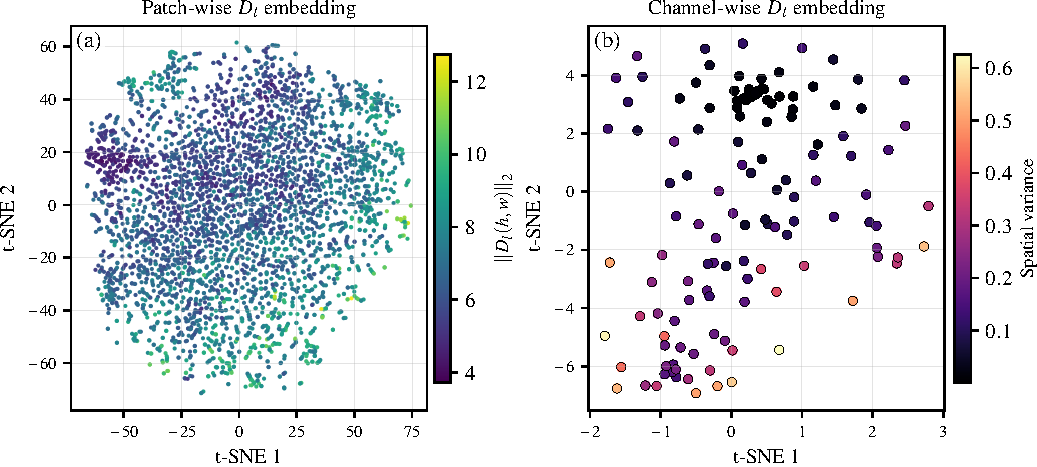
\includegraphics[width=\textwidth,height=0.55\textheight,keepaspectratio]{figures/diagnostics/test1_vanilla_bottleneck_tsne.pdf}
        \end{column}
        \begin{column}{0.42\textwidth}
            \scriptsize
            \[
            \rho=\frac{\|D_l\|_2}{\|X_\Delta\|_2},\qquad
            c=\cos(WX_\Delta,D_l)
            \]
            \begin{tabular}{lrr}
                \toprule
                \textbf{Model} & \(\rho\) & \(c\) \\
                \midrule
                Vanilla & 3.059 & 0.483 \\
                Absolute-only & 0.602 & 0.771 \\
                Signed-only & 0.614 & 0.756 \\
                \bottomrule
            \end{tabular}

            \vspace{0.5em}
            \small
            The vanilla bottleneck is not a passive channel reducer; it strongly re-encodes temporal evidence. This explains why downstream gates and losses matter.
        \end{column}
    \end{columns}
\end{frame}

\begin{frame}{Bottleneck Diagnostic: Channel Activation Hierarchy}
    \begin{columns}[T,onlytextwidth]
        \begin{column}{0.58\textwidth}
            \centering
            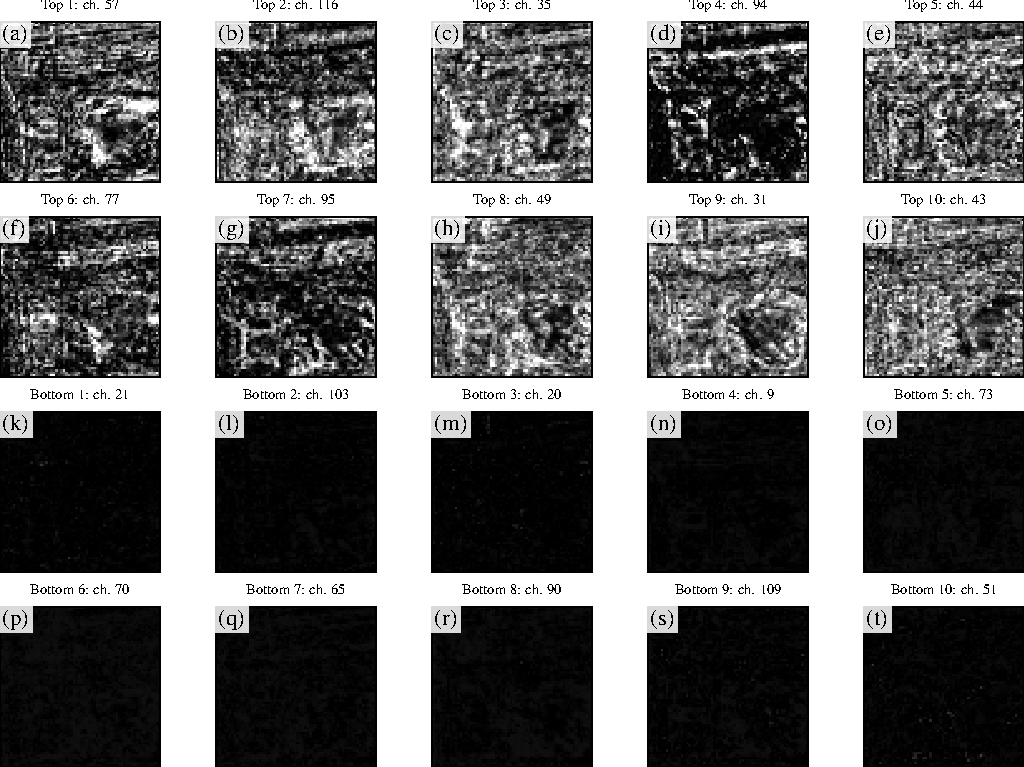
\includegraphics[width=\textwidth,height=0.58\textheight,keepaspectratio]{figures/diagnostics/test2_vanilla_channel_variance_heatmaps.pdf}
        \end{column}
        \begin{column}{0.39\textwidth}
            \scriptsize
            Spatial variance per channel:
            \[
            v_c=\frac{1}{HW}\sum_{i,j}\left(D_{l,cij}-\mu_c\right)^2.
            \]
            \begin{tabular}{lr}
                \toprule
                \textbf{Channel group} & \textbf{Variance range} \\
                \midrule
                Top-10 active & 0.435--0.626 \\
                Bottom-10 quiet & 0.0015--0.0028 \\
                \bottomrule
            \end{tabular}

            \vspace{0.5em}
            \small
            High-variance channels localize structured change evidence. Low-variance channels behave like background suppression or weak context carriers.
        \end{column}
    \end{columns}
\end{frame}

\begin{frame}{Bottleneck Diagnostic: Region and Boundary Gates}
    \centering
    \begin{columns}[T,onlytextwidth]
        \begin{column}{0.49\textwidth}
            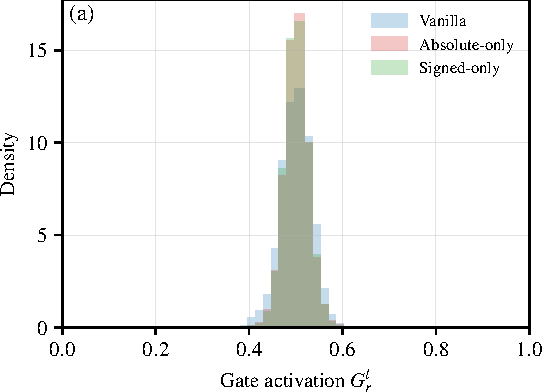
\includegraphics[width=\textwidth,height=0.34\textheight,keepaspectratio]{figures/diagnostics/test3_region_gate_histograms.pdf}
        \end{column}
        \begin{column}{0.49\textwidth}
            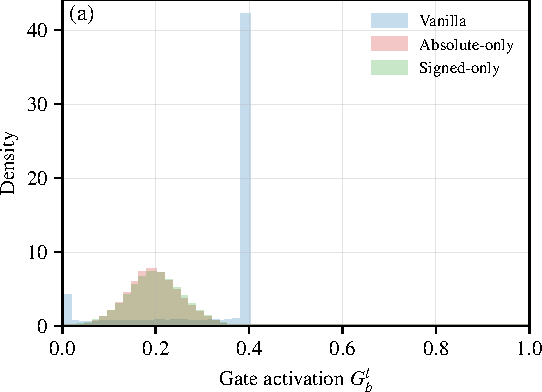
\includegraphics[width=\textwidth,height=0.34\textheight,keepaspectratio]{figures/diagnostics/test3_boundary_gate_histograms.pdf}
        \end{column}
    \end{columns}

    \vspace{0.2em}
    \scriptsize
    \begin{tabular}{lrrrr}
        \toprule
        \textbf{Model / gate} & \textbf{min} & \textbf{max} & \textbf{mean} & \(G<0.05\) \\
        \midrule
        Vanilla \(G_r\) & 0.364 & 0.629 & 0.501 & 0.000 \\
        Vanilla \(G_b\) & 0.000 & 0.400 & 0.329 & 0.086 \\
        Abs-only \(G_b\) & 0.013 & 0.389 & 0.197 & 0.001 \\
        Signed-only \(G_b\) & 0.008 & 0.391 & 0.199 & 0.003 \\
        \bottomrule
    \end{tabular}

    \vspace{0.3em}
    \scriptsize
    Region gates stay centered near 0.5 and do not saturate. Boundary gates are intentionally capped at 0.4, so the boundary path refines rather than dominates the region path.
\end{frame}

\begin{frame}{Experimental Bottlenecks Found in the Archive}
    \small
    \begin{itemize}
        \item \textbf{Boundary residual without boundary supervision:} A4 \(\rightarrow\) A5 decreases F1 and IoU. The residual branch needs edge loss and coarse supervision, not just the main mask loss.
        \item \textbf{Unsigned D-RBI is insufficient:} A1 \(\rightarrow\) A2 drops in the averaged table. Signed temporal evidence recovers and improves the D-RBI path.
        \item \textbf{Backbone scaling saturates:} Small \(\rightarrow\) Base adds \(1.73\times\) parameters for only \(+0.10\) F1.
        \item \textbf{Direct SOTA reproduction was incomplete:} archived jobs hit missing/manual checkpoints, DSIFN dataset-layout mismatch for ChangeFormer, and a WHU CUDA OOM case.
        \item \textbf{Profiling is relative:} fvcore reported unsupported selective-scan and attention operators, so FLOPs are useful for variant scaling but not exact runtime accounting.
        \item \textbf{Legacy result hygiene matters:} wrong-backbone and different-evaluator runs were excluded from canonical averages.
    \end{itemize}
\end{frame}
